% ====================
\chapter{Les boucles}
\label{chap:bcl}
% ====================

	\marginicon{objectif}
	Les ordinateurs révèlent tout leur potentiel dans leur capacité à
	répéter inlassablement les mêmes tâches.
	Nous voyons ici comment incorporer des boucles dans nos codes 
	et comment les utiliser à bon escient.

	\marginicon{attention}
	Attention~! 
	D’expérience, nous savons que ce chapitre est difficile à appréhender. 
	Beaucoup d’entre vous perdent pied ici. 
	Accrochez-vous et faites bien tous les exercices proposés~!

% =======================================
\section{La notion de travail répétitif}
% =======================================

	Si on veut faire effectuer un travail répétitif, 
	il faut indiquer deux choses~:
	
	\begin{enumerate}
	\item Le travail à répéter
	\item La manière de continuer la répétition ou de l’arrêter.
	\end{enumerate}

	Examinons quelques exemples pour fixer notre propos.

	\textbf{Exemple 1}~: 
	Pour traiter des dossiers, 
	on dira quelque chose comme 
	«~tant qu’il reste un dossier à traiter, le traiter~» 
	ou encore 
	«~traiter un dossier puis passer au suivant jusqu’à ce qu’il n’en reste plus à traiter~».

	\begin{liste}
	\item La tâche à répéter est : «~traiter un dossier~»
	\item On indique qu’on doit continuer s’il reste encore un dossier à traiter.
	\end{liste}

	\textbf{Remarque~:}~
	On aurait aussi pu le formuler ainsi~:~
	«~traiter un dossier et passer au suivant jusqu’à ce qu’il n’en reste plus~».

	\textbf{Exemple 2}~:~
	Pour calculer la cote finale de tous les étudiants,
	on aura quelque chose du genre 
	«~Pour tout étudiant, calculer sa cote~».

	\begin{liste}
	\item 
		La tâche à répéter est : «~calculer la cote d’un étudiant~»
	\item 
		On indique qu’on doit le faire pour tous les étudiants.
		On doit donc commencer par le premier, passer à chaque fois au suivant
		et s’arrêter quand on a fini le dernier.
	\end{liste}

	\textbf{Exemple 3}~:~
	Pour afficher tous les nombres de 1 à 100, on aura
	«~Pour tous les nombres de 1 à 100, afficher ce nombre~».

	\begin{liste}
	\item
		La tâche à répéter est : «~afficher un nombre~»
	\item 
		On indique qu’on doit le faire pour tous les nombres de 1 à 100. 
		On doit donc commencer avec 1, 
		passer à chaque fois au nombre suivant 
		et s’arrêter après avoir affiché le nombre 100.
	\end{liste}

	\textbf{Attention}~! 
	Comprenez bien que c’est toujours la même tâche qui est exécutée 
	mais pas avec le même effet à chaque fois. 
	Ainsi, on traite un dossier mais à chaque fois un différent ; 
	on affiche un nombre mais à chaque fois un différent. 
	Nous verrons comment y arriver en algorithmique.

% ==============================
\section{Structures itératives}
% ==============================

	Chacune des structures suivantes traduit une volonté de faire exécuter
	de façon répétée une séquence d’instructions. 

	\subsection{«~tant que~»}

		Le «~tant que~» est une structure qui demande à
		l’exécutant de répéter une tâche (une ou plusieurs
		instructions) tant qu’une condition donnée est vraie.

		\begin{Pseudocode}
		\While{condition}
			\Stmt séquence d’instructions à exécuter
		\EndWhile
		\end{Pseudocode}

		Comme pour la structure \pseudocode{si}, 
		la \pseudocode{condition} est une expression à valeur booléenne. 
		Dans ce type de structure, 
		il faut qu’il y ait dans la séquence d’instructions comprise entre
		\pseudocode{tant que} et \pseudocode{fin tant que} au moins une
		instruction qui modifie une des composantes de la condition de telle
		manière qu’elle puisse devenir \textbf{fausse} à un moment donné. Dans
		le cas contraire, la condition reste indéfiniment vraie et la boucle va
		tourner sans fin, c’est ce qu’on appelle une \textbf{boucle infinie}. 
		La figure \vref{fig:boucle-tq} est un ordinogramme 
		décrivant le déroulement de cette structure. 
		On remarquera que si la condition est fausse dès le début, 
		la tâche n’est jamais exécutée.

		\begin{figure}[h]
		\centering
		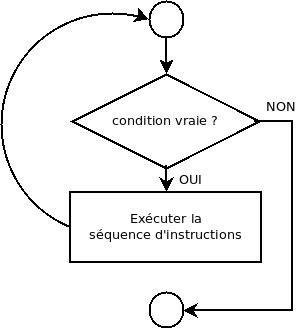
\includegraphics[width=0.5\textwidth]{image/boucle-tq}
		\caption{Ordinogramme de la boucle "tant-que"}
		\label{fig:boucle-tq}
		\end{figure}
		
	\subsection{«~faire~–~jusqu’à ce que~»}

		Cette structure est très proche du «~tant que~» 
		à deux différences près~:
	
		\begin{enumerate}
		\item
			Le test est fait à la fin et pas au début. 
			La tâche est donc toujours exécutée au moins une fois.
		\item 
			On donne la condition pour arrêter et pas pour continuer ; 
			il s’agit d’une différence mineure.
		\end{enumerate}

		\begin{Pseudocode}
		\Repeat
			\Stmt séquence d’instructions à exécuter
		\Until{condition}
		\end{Pseudocode}

		Comme ci-dessus, il faut que la séquence d’instructions comprise entre
		\pseudocode{faire} et \pseudocode{jusqu’à ce que} 
		contienne au moins une instruction qui modifie la condition de
		telle manière qu’elle puisse devenir \textbf{vraie} à un moment donné
		pour arrêter l’itération. 
		La figure \vref{fig:boucle-faire} décrit le déroulement de cette boucle. 

		\begin{figure}[h]
		\centering
		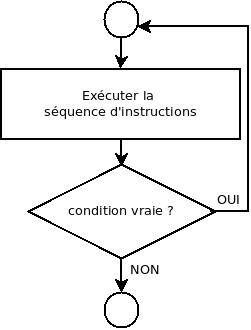
\includegraphics[width=0.4\textwidth]{image/boucle-faire}
		\caption{Ordinogramme de la boucle "faire – jusqu’à ce que"}
		\label{fig:boucle-faire}
		\end{figure}

	\subsection{«~pour~»}

		Ici, on va plutôt indiquer \textbf{combien de fois} la tâche doit être
		répétée. Cela se fait au travers d’une
		\textbf{variable de contrôle} dont la valeur va évoluer à partir
		d’une valeur de départ jusqu’à une
		valeur finale.
		
		\begin{Pseudocode}
		\For{variable \K{de} début \K{à} fin [\K{par} pas]}
			\Stmt séquence d’instructions à exécuter
		\EndFor
		\end{Pseudocode}

		Dans ce type de structure, 
		\pseudocode{début}, \pseudocode{fin} et \pseudocode{pas}
		peuvent être des constantes, des variables ou des expressions 
		(le plus souvent à valeurs entières mais on admettra parfois des réels). 
		Le \pseudocode{pas} est facultatif, et généralement omis 
		(dans ce cas, sa valeur par défaut est 1). 
		Ce pas est parfois négatif, dans le cas d’un compte à rebours, 
		par exemple \pseudocode{pour n de 10 à 1 par -1}.

		Quand le \pseudocode{pas} est positif, la boucle s’arrête
		lorsque la variable dépasse la valeur de \pseudocode{fin}. 
		Par contre, avec un \pseudocode{pas} négatif, 
		la boucle s’arrête lorsque la variable prend une valeur 
		plus petite que la valeur de \pseudocode{fin}
		(cf. le test dans l’organigramme de la figure \vref{fig:boucle-pour}).

		\begin{figure}[h]
		\centering
		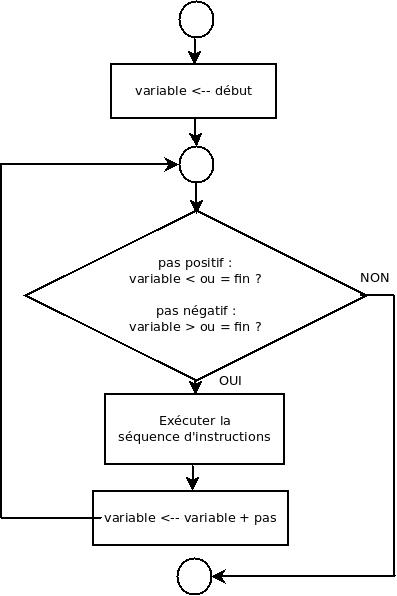
\includegraphics[width=0.5\textwidth]{image/boucle-pour}
		\caption{Ordinogramme de la boucle "pour"}
		\label{fig:boucle-pour}
		\end{figure}

		\marginicon{attention}
		Veiller à la cohérence de l’écriture de cette structure. On considérera
		qu’au cas (à éviter) où \pseudocode{début} est strictement supérieur à
		\pseudocode{fin} et le \pseudocode{pas} est positif, la séquence d’instructions
		n’est jamais exécutée (mais ce n’est pas le cas dans tous les langages
		de programmation~!). Idem si \pseudocode{début} est strictement inférieur à
		\pseudocode{fin} mais avec un \pseudocode{pas} négatif.

		\textbf{Exemples~}:

		\begin{Pseudocode}
		\Stmt \K{pour} i \K{de} 0 \K{à} 2 \K{faire} \RComment La boucle est exécutée 3 fois.
		\Stmt \K{pour} i \K{de} 2 \K{à} 0 \K{faire} \RComment La boucle n’est pas exécutée.
		\Stmt \K{pour} i \K{de} 1 \K{à} 10 \K{par} -1 \K{faire} \RComment La boucle n’est pas exécutée.
		\Stmt \K{pour} i \K{de} 1 \K{à} 1 \K{par} 5 \K{faire} \RComment La boucle est exécutée 1 fois.
		\end{Pseudocode}
		
		\marginicon{attention}
		Veiller aussi à ne pas modifier dans la séquence d’instructions une des
		variables de contrôle \pseudocode{début}, \pseudocode{fin} ou \pseudocode{pas}~! Il
		est aussi fortement déconseillé de modifier «~manuellement~» la
		\pseudocode{variable} de contrôle au sein de la boucle
		\pseudocode{pour}. Il ne faut pas l’initialiser en début de boucle,
		et ne pas s’occuper de sa modification, l’instruction 
		\pseudocode{variable \Gets variable + pas} 
		étant automatique et implicite à chaque étape de la
		boucle. Il est aussi déconseillé d’utiliser \pseudocode{variable} à la
		sortie de la structure \pseudocode{pour} sans lui affecter une
		nouvelle valeur (son contenu pouvant varier selon le langage de
		programmation).

	\subsection{Quel type de boucle choisir~?}

		En pratique, il est possible d’utiliser systématiquement la boucle 
		\pseudocode{tant que} qui peut s’adapter à toutes les situations. 
		Cependant, il est plus clair d’utiliser la boucle \pseudocode{pour} 
		dans les cas où le nombre d’itérations est fixé et connu à l’avance 
		(par là, on veut dire que le nombre d’itérations est déterminé au moment 
		où on arrive à la boucle). 
		La boucle \pseudocode{faire} convient quant à elle
		dans les cas où le contenu de la boucle doit être parcouru au moins une
		fois, alors que dans \pseudocode{tant que}, 
		le nombre de parcours peut être nul si la condition initiale est fausse. 
		La figure \vref{fig:boucle-choix} propose un petit schéma récapitulatif.

		\begin{figure}[h]
		\centering
		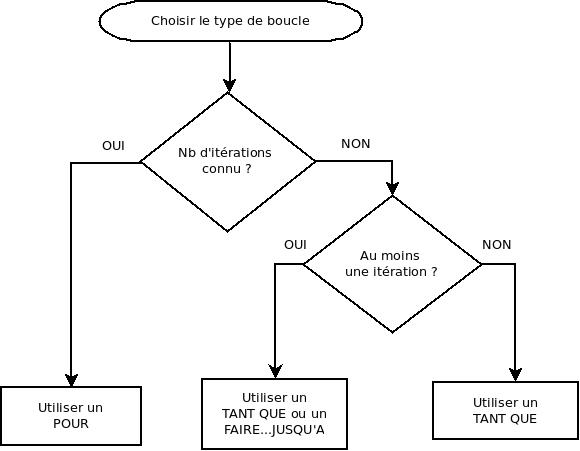
\includegraphics[width=0.8\textwidth]{image/boucle-choixtype}
		\caption{Quel type de boucle choisir~?}
		\label{fig:boucle-choix}
		\end{figure}

% =================
\section{Exemples}
% =================

	Nous présentons quelques exemples de difficulté
	croissante pour montrer comment bien utiliser les boucles.

	\subsection{Exemple 1 -- Compter de 1 à 10}

		Imaginons qu’on veuille afficher tous les nombres de 1 à 10. 
		On va évidemment rejeter cette première solution~:

		\begin{Pseudocode}
		\LComment Affiche les nombres de 1 à 10.
		\Module{compterJusque10}{}{} \RComment une mauvaise solution !
		\Write 1
		\Write 2
		\Write 3
		\Write 4
		\Write 5
		\Write 6
		\Write 7
		\Write 8
		\Write 9
		\Write 10
		\EndModule
		\end{Pseudocode}

		Non seulement c’est long à écrire 
		(imaginer l’algorithme pour afficher les nombres de 1 à 10000~!) 
		mais c’est très peu souple.
		Cela ne fonctionne que pour 10~:~il faut modifier l’algorithme pour
		un autre comptage. La boucle va nous permettre
		d’obtenir un algorithme qui s’adapte
		à la limite du décompte.

		Posons-nous les bonnes questions pour déterminer la boucle~:

		\begin{liste}
		\item 
			Quelle est la tâche à répéter~? Afficher un nombre.
		\item 
			Comment savoir si on continue~? On arrête quand «~10~» est affiché.
		\item 
			Comment afficher à chaque fois un nombre différent~? 
			Au travers d’une variable qui prendra toutes les valeurs de 1 à 10. 
			Il faut donc ajouter dans le corps de la
			boucle une incrémentation de la variable
		\end{liste}

		Ce qui donne~:

		\begin{Pseudocode}
		\LComment Affiche les nombres de 1 à 10.
		\Module{compterJusque10}{}{} \RComment version avec tant que
			\Decl nb : entier
			\Let nb \Gets 1 \RComment c’est le premier nombre à afficher
			\While{nb $\leq$ 10} \RComment tant que le nb à afficher est toujours bon
				\Write nb \RComment on affiche la valeur de la variable nb
				\Let nb \Gets nb + 1 \RComment on passe au nombre suivant
			\EndWhile
		\EndModule
		\end{Pseudocode}

		Mais ici, on pourrait aussi l’écrire avec un «~pour~» vu qu’on
		connait exactement le nombre d’exécutions de la boucle (10). 
		La variable de contrôle va évoluer de 1 à 10 ce qui tombe bien car
		c’est justement le nombre à afficher à chaque fois.

		\begin{Pseudocode}
		\LComment Affiche les nombres de 1 à 10.
		\Module{compterJusque10}{}{} \RComment version avec pour
			\Decl nb : entier
			\For{nb \K{de} 1 \K{à} 10} \RComment par défaut le pas est de 1
				\Write nb 
			\EndFor
		\EndModule
		\end{Pseudocode}

		On obtient une solution plus courte et plus lisible 
		car l’en-tête du «~pour~» indique clairement
		comment va évoluer la boucle
		(valeur de départ, pas et valeur finale)

	\subsection{Exemple 2 -- Compter de 1 à beaucoup}

		Dans l’exercice précédent, on a
		affirmé que la boucle pouvait s’adapter à la limite du
		décompte. Montrons-le~! Supposons qu’on veuille
		afficher les nombres de 1 à $n$ où $n$ est une valeur 
		donnée par l’utilisateur.

		Rien de plus simple, il suffit de lire cette
		valeur au début et de l’utiliser comme limite de boucle

		\begin{Pseudocode}
		\LComment Lit un nombre et affiche les nombres de 1 à ce nombre.
		\Module{afficherN}{}{} 
			\Decl nb, n : entier
			\Read n
			\For{nb \K{de} 1 \K{à} n} 
				\Write nb 
			\EndFor
		\EndModule
		\end{Pseudocode}

		\marginicon{reflexion}
		\textbf{Réflexion}~: Que se passe-t-il si l’utilisateur entre une valeur négative~?
		Comment améliorer le code pour que le programme
		le signale à l’utilisateur~?

	\subsection{Exemple 3 -- Afficher les nombres pairs}

		Cela se complique un peu. Cette fois-ci on
		affiche uniquement les nombres \textbf{pairs} jusqu’à la limite $n$.
		
		\textbf{Exemple}~:~les nombres pairs de $1$ à $10$ sont~: $2$, $4$, $6$, $8$, $10$.
		
		Notez que $n$ peut être impair. Si $n$ vaut $11$, 
		l’affichage est le même que pour $10$.

		Est-ce qu’on peut utiliser un «~pour~»~? 
		Oui. De 1 à $n$, il y a exactement «~$n$ DIV $2$~» nombres à afficher. 
		La difficulté vient du lien à faire entre la variable de
		contrôle et le nombre à afficher.

		\textbf{Solution 1}~:~on garde le lien entre la variable de contrôle 
		et le nombre à afficher. 
		Dans ce cas, on commence à $2$ et le pas doit être de $2$.

		\begin{Pseudocode}
		\LComment Lit un nombre et affiche les nombres pairs jusqu’à ce nombre.
		\Module{afficherPair}{}{} 
			\Decl nb, n : entier
			\Read n
			\RComment limite des nombres à afficher
			\For{nb \K{de} 2 \K{à} n \K{par} 2} 
				\Write nb 
			\EndFor
		\EndModule
		\end{Pseudocode}

		\textbf{Solution 2}~:~la variable de contrôle compte simplement 
		le nombre d’itérations.
		Alors il faut calculer le nombre à afficher en fonction de la variable
		de contrôle (ici le double de celle-ci convient)

		\begin{Pseudocode}
		\LComment Lit un nombre et affiche les nombres pairs jusqu’à ce nombre.
		\Module{afficherPair}{}{} 
			\Decl i, n : entier
			\Read n
			\RComment limite des nombres à afficher
			\For{i \K{de} 1 \K{à} n DIV 2} 
				\Write 2 * i 
			\EndFor
		\EndModule
		\end{Pseudocode}

		Par une vieille habitude des programmeurs%
		\footnote{%
			Née avec le langage FORTRAN 
			où la variable $i$ était par défaut une variable entière.
		},
		une variable de contrôle qui se contente de compter les passages dans
		la boucle est souvent nommée $i$. 
		On l’appelle aussi «~itérateur~».

	\subsection{Exemple 4 -- Afficher les premiers nombres pairs}

		Voici un problème proche du précédent~:~on affiche cette fois 
		les $n$ premiers nombres pairs.
		
		\textbf{Exemple}~:~les $10$ premiers nombres pairs sont~:~$2$, $4$, $6$, $8$, 
		$10$, $12$, $14$, $16$, $18$, $20$.
		
		Il est plus simple de partir de la solution 2 de l’exemple précédent
		en changeant simplement la valeur finale de la boucle.

		\begin{Pseudocode}
		\LComment Lit un nombre et affiche ce nombre de nombres pairs.
		\Module{afficherPair}{}{} 
			\Decl i, n : entier
			\Read n
			\RComment le nombre de nombres à afficher
			\For{i \K{de} 1 \K{à} n} 
				\Write 2 * i 
			\EndFor
		\EndModule
		\end{Pseudocode}

	\subsection{Exemple 5 -- Somme de nombres}

		Changeons de problème. On veut pouvoir calculer (et retourner)
		la somme d’une série de nombres donnés par
		l’utilisateur. Il faut d’abord se
		demander comment l’utilisateur va pouvoir indiquer
		combien de nombres il faut additionner ou quand est-ce que le dernier
		nombre à additionner a été entré. Voyons quelques possibilités.

		\medskip
		\textbf{Variante 1}~: 
		
		L’utilisateur indique le nombre de termes au départ.
		Ce problème est proche de ce qui a déjà été fait.
		
		\begin{Pseudocode}
		\LComment Lit des valeurs entières et retourne la somme des valeurs lues.
		\Module{sommeNombres}{}{entier} \RComment Variante 1
			\Decl nbValeurs : entier \RComment nb de valeurs à additionner
			\Decl valeur : entier \RComment un des termes de l’addition
			\Decl somme : entier \RComment la somme
			\Decl i : entier \RComment itérateur
			\Let somme \Gets 0 \RComment la somme se construit petit à petit. 0 au départ
			\Read nbValeurs
			\For{i \K{de} 1 \K{à} nbValeurs} 
				\Read valeur
				\Let somme \Gets somme + valeur 
			\EndFor
			\Return somme
		\EndModule
		\end{Pseudocode}

		\medskip
		\textbf{Variante 2}~: 
		
		Après chaque nombre, 
		on demande à l’utilisateur s’il y a encore un nombre à additionner.

		Ici, il faut chercher une solution différente
		car on ne connait pas au départ le nombre de valeurs à additionner et
		donc le nombre d’exécution de la boucle. On va devoir passer à un
		«~tant que~» ou un «faire - jusqu’à ce que». On peut
		envisager de demander en fin de boucle s’il reste
		encore un nombre à additionner. Ce qui donne~:

		\begin{Pseudocode}
		\LComment Lit des valeurs entières et retourne la somme des valeurs lues.
		\Module{sommeNombres}{}{entier} \RComment Variante 2a
			\Decl encore : booléen \RComment est-ce qu’il reste encore une valeur à additionner~?
			\Decl valeur : entier \RComment un des termes de l’addition
			\Decl somme : entier \RComment la somme
			\Let somme \Gets 0
			\Repeat 
				\Read valeur
				\Let somme \Gets somme + valeur 
				\Read encore
			\Until{NON encore}
			\Return somme
		\EndModule
		\end{Pseudocode}
		
		Avec cette solution, on additionne au moins une valeur. 
		Si on veut pouvoir tenir compte du
		cas très particulier où l’utilisateur ne veut
		additionner aucune valeur, il faut utiliser un «~tant que~» et donc
		poser la question avant d’entrer dans la boucle.

		\begin{Pseudocode}
		\LComment Lit des valeurs entières et retourne la somme des valeurs lues.
		\Module{sommeNombres}{}{entier} \RComment Variante 2b
			\Decl encore : booléen \RComment est-ce qu’il reste encore une valeur à additionner~?
			\Decl valeur : entier \RComment un des termes de l’addition
			\Decl somme : entier \RComment la somme
			\Let somme \Gets 0
			\Read encore
			\While{encore} 
				\Read valeur
				\Let somme \Gets somme + valeur 
				\Read encore
			\EndWhile
			\Return somme
		\EndModule
		\end{Pseudocode}

		\medskip
		\textbf{Variante 3}~:
		
		L’utilisateur entre une valeur spéciale pour indiquer la fin. 
		On parle de valeur \textbf{sentinelle}. 
		Ceci n’est possible que si cette valeur \textbf{sentinelle} ne peut pas être
		un terme valide de l’addition. Par exemple, si on veut
		additionner des nombres positifs uniquement, la valeur -1 peut servir
		de valeur sentinelle. Mais sans limite sur les nombres à additionner
		(positifs, négatifs ou nuls) il n’est pas possible de
		choisir une sentinelle.

		Ici, on se base sur la valeur entrée pour décider si on continue ou pas. 
		Il faut donc \textbf{toujours} effectuer un test
		après une lecture de valeur. C’est pour cela
		qu’il faut effectuer une lecture avant et une autre à
		la fin de la boucle.

		\begin{Pseudocode}
		\LComment Lit des valeurs entières et retourne la somme des valeurs lues.
		\Module{sommeNombres}{}{entier} \RComment Variante 3
			\Decl valeur : entier \RComment un des termes de l’addition
			\Decl somme : entier \RComment la somme
			\Let somme \Gets 0
			\Read valeur
			\While{valeur ${\geq}$ 0} 
				\Let somme \Gets somme + valeur 
				\Read valeur \RComment remarquer l’endroit où on lit une valeur.
			\EndWhile
			\Return somme
		\EndModule
		\end{Pseudocode}

		\marginicon{reflexion}
		\textbf{Réflexions}~: 
		\begin{liste}
		\item
			Quelle valeur sentinelle prendrait-on 
			pour additionner une série de cotes d’interrogations~? 
			Une série de températures~?
		\item
			Dans les solutions 2 et 3 on lit une variable booléenne. 
			Comment un programmeur pourrait-il réaliser 
			cette instruction de façon pratique~?		
		\end{liste}
		
	\subsection{Exemple 6~:~Suite des nombres pairs}

		Ce chapitre propose en exercice des suites.
		Toutes ces suites peuvent se résoudre 
		en suivant un même squelette d’algorithme 
		que nous allons expliquer ici.
	
		Un exemple simple pourrait être celui-ci~:
		\og{}Écrire l’algorithme qui affiche les $n$ premiers termes
		de la suite: $2$, $4$, $6$\dots\fg{}
	
		Puisqu’on doit écrire plusieurs nombres et qu’on sait exactement combien,
		on se tournera tout naturellement vers une boucle \K{pour}.
		
		Le cas le plus simple est lorsque le nombre à afficher à l’étape $i$
		peut être calculé en fonction de $i$ seulement.
		L’algorithme est alors
		
		\begin{Pseudocode}
		\For{i de 1 à n}
			\Write $f(i)$
		\EndFor
		\end{Pseudocode}
		
		Dans ce cas, la fonction est $f(i)=2*i$
		(Si vous n’êtes pas convaincu, vérifiez qu’à l’étape $1$ on affiche $2$,
		à l’étape $2$ on affiche $4$\dots) ce qui donne
		
		\begin{Pseudocode}
		\Module{nombrePair}{n\In : entier}{}
			\Decl i : entier
			\For{i de 1 à n}
				\Write 2 * i
			\EndFor
		\EndModule
		\end{Pseudocode}
		
		Parfois, il est difficile (voire impossible) de trouver $f(i)$.
		On suivra alors une autre approche qui revient à calculer un nombre
		à afficher à partir du nombre précédemment affiché
		(ou, plus exactement, de calculer le suivant à partir du nombre
		qu’on vient d’afficher).
		La structure générale est alors
		
		\begin{Pseudocode}
		\Let nb \Gets \textit{\{1\up{ère} valeur à afficher\}}
		\For{i de 1 à n}
			\Write nb
			\Let nb \Gets \textit{\{calculer ici le nb suivant\}}
		\EndFor
		\end{Pseudocode}
		
		Dans l’exemple de la suite paire, le 1\up{er} nombre à afficher est $2$
		et le nombre suivant se calcule en ajoutant $2$ au nombre courant.
		
		\begin{Pseudocode}
		\Module{suite1}{n\In : entier}{}
			\Decl nb, i : entiers
			\Let nb \Gets 2
			\For{i de 1 à n}
				\Write nb
				\Let nb \Gets nb + 2
			\EndFor
		\EndModule
		\end{Pseudocode}
		
		On remarque que, lors du dernier passage dans la boucle,
		on calcule une valeur qui ne sera pas affichée.
		Cette petite perte de temps est dommage mais négligeable
		et permet de garder une structure claire et générale à la solution.
		
		Dans certains cas,
		il n’est pas possible de déduire directement le nombre suivant
		en connaissant juste le nombre précédent.
		Prenons un exemple un peu plus compliqué pour l’illustrer.
		
	\subsection{Exemple 7~:~3 pas en avant, 2 pas en arrière} 
	
		Compliquons un peu~: 
		\og{}Écrire l’algorithme qui affiche les $n$ premiers termes
		de la suite~:~$1$, $2$, $3$, $4$, $3$, $2$, $3$, $4$, $5$, $4$, $3$\dots\fg{}
	
		Si on vient d’écrire, disons un $3$,
		impossible sans information supplémentaire,
		de connaitre le nombre suivant.
		Il faudrait savoir si on est en phase d’avancement ou de recul
		et combien de pas il reste à faire dans cette direction.
		
		Ajoutons des variables pour retenir l’\emph{état} où on est.
		
		\begin{Pseudocode}
		\Module{suite3Avant2Arrière}{n\In : entier}{} 
			\Decl nb, nbPasRestants, direction, i : entiers
			\Let nb \Gets 1
			\Let nbPasRestants \Gets 3 \RComment 3 pas
			\Let direction \Gets 1 \RComment en avant
			\For{i de 1 à n}
				\Write nb
				\Let nb \Gets nb + direction \RComment faire un pas dans la bonne direction
				\Let nbPasRestants \Gets nbPasRestants - 1
				\If{nbPasRestants $=$ 0} \RComment il est temps de changer de direction
					\Let direction \Gets -direction
					\If{direction $=$ 1}
						\Let nbPasRestants \Gets 3 
					\Else 
						\Let nbPasRestants \Gets 2
					\EndIf
				\EndIf
			\EndFor
		\EndModule
		\end{Pseudocode}
		
		On obtient un algorithme plus long 
		mais qui respecte toujours le schéma vu.
		
		\textbf{Un conseil}~:~essayez de respecter ce schéma 
		et vous obtiendrez plus facilement un algorithme
		correct et lisible, également dans les cas particuliers.
	
% ==================
\section{Exercices}
% ==================

	Voilà~! Vous devriez à présent être en mesure de
	résoudre les exercices qui suivent.
	Courage~! Et n’en passez aucun~!

\begin{Exercice}{Compréhension d’algorithmes}
	Quels sont les affichages réalisés lors de l’exécution
	des algorithmes suivants~?
	
	\begin{Pseudocode}
	\Module{boucle1}{}{}
		\Decl x : entier
		\Let x \Gets 0
		\While{x < 12}
			\Let x \Gets x + 2	
		\EndWhile
		\Write x
	\EndModule
	\end{Pseudocode}

	\begin{Pseudocode}
	\Module{boucle2}{}{}
		\Decl ok : booléen
		\Decl x : entier
		\Let ok \Gets vrai
		\Let x \Gets 5
		\While{ok}
			\Let x \Gets x + 7	
			\Let ok \Gets x MOD 11 $\neq$ 0	
		\EndWhile
		\Write x
	\EndModule
	\end{Pseudocode}

	\begin{Pseudocode}
	\Module{boucle3}{}{}
		\Decl ok : booléen
		\Decl cpt, x : entiers
		\Let x \Gets 10
		\Let cpt \Gets 0
		\Let ok \Gets vrai
		\While{ok ET cpt < 3}
			\If{x MOD 2 = 0}
				\Let x \Gets x + 1
				\Let ok \Gets x < 20
			\Else
				\Let x \Gets x + 3
				\Let cpt \Gets cpt + 1
			\EndIf
		\EndWhile
		\Write x
	\EndModule
	\end{Pseudocode}

	\begin{Pseudocode}
	\Module{boucle4}{}{}
		\Decl pair, grand : booléens
		\Decl p, x : entiers
		\Let x \Gets 1
		\Let p \Gets 1
		\Repeat
			\Let p \Gets 2 * p
			\Let x \Gets x + p
			\Let pair \Gets x MOD 2 = 0
			\Let grand \Gets x > 15
		\Until{pair OU grand}
		\Write x
	\EndModule
	\end{Pseudocode}

	\begin{Pseudocode}
	\Module{boucle5}{}{}
		\Decl i, x : entiers
		\Decl ok : booléen
		\Let x \Gets 3
		\Let ok \Gets vrai
		\For{i \K{de} 1 \K{à} 5}
			\Let x \Gets x + i
			\Let ok \Gets ok ET (x MOD 2 = 0)
		\EndFor
		\If{ok}
			\Write x
		\Else
			\Write 2 * x
		\EndIf
	\EndModule
	\end{Pseudocode}

	\begin{Pseudocode}
	\Module{boucle6}{}{}
		\Decl i, j, fin : entiers
		\For{i \K{de} 1 \K{à} 3}
			\Let fin \Gets 6 * i - 11
			\For{j \K{de} 1 \K{à} fin \K{par} 3}
				\Write 10 * i + j
			\EndFor
		\EndFor
	\EndModule
	\end{Pseudocode}
\end{Exercice}

\begin{Exercice}{Simplification}
	Voici quelques extraits d’algorithmes corrects du point de vue de la
	syntaxe mais contenant des lignes inutiles ou des lourdeurs d’écriture.
	Remplacez ces portions d’algorithme par un minimum d’instructions qui
	auront un effet équivalent.

	\begin{Pseudocode}
	\Let a \Gets 1
	\Let b \Gets 1
	\While{a < 10}
		\Let a \Gets a + 1
		\Let b \Gets b + 1
		\Write b
	\EndWhile
	\end{Pseudocode}

	\begin{Pseudocode}
	\Let a \Gets 1
	\Let b \Gets 1
	\While{a < 10}
		\Let a \Gets a + 1
		\Let b \Gets b + 1
	\EndWhile
	\Write b
	\end{Pseudocode}

	\begin{Pseudocode}
	\Let i \Gets 1
	\For{i \K{de} 1 \K{à} 10}
		\Let b \Gets i
	\EndFor
	\end{Pseudocode}
\end{Exercice}

\begin{Exercice}{Afficher les n premiers}
	Écrire un algorithme qui lit un naturel $n$ et affiche
	
	\begin{liste}
	\item {
	les $n$ premiers entiers strictement positifs ;}
	\item {
	les $n$ premiers entiers strictement positifs en ordre décroissant ;}
	\item {
	les $n$ premiers carrés parfaits ;}
	\item {
	les $n$ premiers naturels impairs ;}
	\item {
	les naturels impairs qui sont inférieurs ou égaux à $n$.}
	\end{liste}
\end{Exercice}

\begin{Exercice}{Maximum de nombres}
	Écrire un algorithme qui lit une série de cotes d’interrogation (entiers
	entre 0 et 20) et affiche ensuite la plus grande. Pour signaler la fin
	de l’encodage des cotes, l’utilisateur introduit un nombre négatif
	(\textbf{valeur sentinelle}).
\end{Exercice}

\begin{Exercice}{Afficher les multiples de 3}
	Écrire un algorithme qui lit une série de nombres entiers positifs,
	jusqu’à ce que l’utilisateur encode la valeur 0. Les nombres multiples
	de 3 seront affichés au fur et à mesure et le nombre de ces multiples
	sera affiché en fin de traitement.
\end{Exercice}

\begin{Exercice}{Placement d’un capital}
	On placera le 1\up{er} janvier de l’année à venir un
	capital pendant un certain nombre d’années à un certain taux. Le
	capital évolue suivant le système des intérêts composés. Écrire un
	algorithme qui, à partir du capital de départ, du nombre d’années et du
	taux de placement (en \%), affiche pour chaque année les informations
	suivantes~:~la date, le capital et les intérêts obtenus au
	1\up{er} janvier de cette année.
\end{Exercice}

\bigskip
\begin{Exercice}{Produit de 2 nombres}
	Écrire un algorithme qui retourne le produit de deux entiers quelconques
	sans utiliser l’opérateur de multiplication, mais en minimisant le
	nombre d’opérations.
\end{Exercice}

\begin{Exercice}{Génération de suites}
	\marginicon{java}
	Écrire un algorithme qui affiche les \textbf{$n$ premiers termes} des
	suites suivantes~:

	\begin{enumerate}[label=\alph*)]
	\item {Le pas croissant 
	
	1, 2, 4, 7, 11, 16, \dots}
	\item {La boiteuse
	
	1, 2, 4, 5, 7, 8, 10, 11, \dots}
	\item {La suite de Fibonacci
	
	0, 1, 1, 2, 3, 5, 8, 13, 21, \dots }
	\item {La procession d’Echternach
	
	1, 2, 3, 4, 3, 2, 3, 4, 5, 4, 3, 4, 5, 6, 5, 4, 5, 6, \dots}
	\item {La combinaison de deux suites
	
	1, 2, 3, 3, 5, 4, 7, 5, 9, 6, 11, 7, 13, 8, \dots }
	\item {La capricieuse
	
	1, 2, 3, 4, 5, 6, 7, 8, 9, 10, 20, 19, 18, 17, 16, 15, 14, 13, 12, 11,
	21, 22, 23, 24, 25, 26, 27, 28, 29, 30, 40, 39, 38, \dots, 31, 41, 42, \dots}
	\end{enumerate}
\end{Exercice}

\begin{Exercice}{Factorielle}
	Écrire un algorithme qui retourne la factorielle de $n$ (entier positif ou
	nul). Rappel~: la factorielle de $n$, notée $n$!, est le produit des $n$
	premiers entiers strictement positifs. 
	
	Par convention, 0! = 1.
\end{Exercice}

\begin{Exercice}{Somme de chiffres}
	\marginicon{java}
	Écrire un algorithme qui retourne la somme des chiffres qui forment un
	nombre naturel $n$. Attention, on donne au départ \textbf{le} nombre et
	pas ses chiffres. Exemple~: 133045 doit donner comme résultat 16,
	car 1 + 3 + 3 + 0 + 4 + 5 = 16.
\end{Exercice}

\begin{Exercice}{Conversion binaire-décimale}
	\marginicon{java}
	Écrire un algorithme qui lit un nombre entier positif censé représenter
	une configuration binaire (et donc ne contenant que des chiffres 0 et
	1) et qui retourne la conversion de ce nombre en base 10. Attention, on
	lit \textbf{un} nombre et on affiche \textbf{un} nombre. Améliorer
	l’algorithme de sorte qu’il signale une éventuelle erreur d’encodage.
\end{Exercice}

\begin{Exercice}{Conversion décimale-binaire}
	Écrire un algorithme qui lit un entier positif et retourne sa
	configuration binaire.
\end{Exercice}

\begin{Exercice}{PGCD}
	Écrire un algorithme qui calcule le PGCD (plus grand commun diviseur) de
	deux entiers positifs selon l’algorithme d’Euclide.
\end{Exercice}

\begin{Exercice}{PPCM}
	Écrire un algorithme qui calcule le PPCM (plus petit commun multiple) de
	deux entiers positifs.
\end{Exercice}

\begin{Exercice}{Nombre premier}
	Écrire un algorithme qui vérifie si un entier positif est un
	\textbf{nombre premier}. 
	
	Rappel~:~un nombre est premier s’il n’est divisible que par 1 et par
	lui-même. Le premier nombre premier est 2.
\end{Exercice}

\bigskip
\begin{Exercice}{Nombres premiers}
	Écrire un algorithme qui affiche les nombres premiers inférieurs ou
	égaux à un entier positif donné. Le module de cet algorithme fera appel
	de manière répétée mais économique à celui de l’exercice précédent.
\end{Exercice}

\begin{Exercice}{Nombre parfait}
	Écrire un algorithme qui vérifie si un entier positif est un
	\textbf{nombre parfait}, c’est-à-dire un nombre égal à la somme de ses
	diviseurs (sauf lui-même). 
	
	Par exemple, 6 est parfait car 6 = 1 + 2 + 3. 
	
	De même, 28 est parfait car 28 = 1 + 2 + 4 + 7 + 14.
\end{Exercice}

\begin{Exercice}{Décomposition en facteurs premiers}
	Écrire un algorithme qui affiche la décomposition 
	d’un entier en facteurs premiers. 
	Par exemple, $1001880$ donnerait comme décomposition
	$2^3 * 3^2 * 5 * 11^2 * 23$.
\end{Exercice}

\begin{Exercice}{Palindrome}
	Écrire un algorithme qui vérifie si un entier donné 
	forme un palindrome ou non. 
	Un nombre palindrome est un nombre qui lu dans un sens 
	(de gauche à droite) est identique au nombre lu dans l’autre sens 
	(de droite à gauche). 
	Par exemple, $1047401$ est un nombre palindrome.
\end{Exercice}

\begin{Exercice}{Jeu de la fourchette}
	\marginicon{java}
	Écrire un algorithme qui simule le jeu de la
	fourchette. Ce jeu consiste à essayer de découvrir un nombre quelconque
	compris entre 1 et 100 inclus, tiré au sort par l’ordinateur (la primitive
	\pseudocode{hasard(n~:~entier)} retourne un entier entre 1 et $n$). 
	L’utilisateur a droit à huit essais
	maximum. À chaque essai, l’algorithme devra afficher un message
	indicatif «~nombre donné trop petit~» ou «~nombre donné trop grand~».
	En conclusion, soit «~bravo, vous avez trouvé en [nombre] essai(s)~» soit
	«~désolé, le nombre était [valeur]~».
\end{Exercice}

\begin{Exercice}{IMC}
	L’IMC (\textit{Indice de Masse Corporelle}) est une mesure permettant à
	chacun d’entre nous de se situer sur une échelle de corpulence. On
	obtient l’IMC en divisant le poids en kilo par le carré de la taille en
	mètre. 
	
	La catégorie de corpulence en fonction de l’IMC est donnée par le tableau 
	suivant~:
	
	\begin{center}
		\begin{tabular}{|*{3}{>{\centering\arraybackslash}m{4cm}|}}
			\hline
			\textbf{Corpulence} & \textbf{IMC homme} & \textbf{IMC femme} 
			\\\hline\hline
			maigre & strictement moins de 20 & strictement moins de 19
			\\\hline
			normal & entre 20 et 25 inclus & entre 19 et 24 inclus
			\\\hline
			excès pondéral & entre 25 exclu et 30 inclus & entre 24 exclu et 30 inclus
			\\\hline
			obèse & plus de 30 & plus de 30
			\\\hline
		\end{tabular}
	\end{center}
	
	Écrire un algorithme qui lit les données d’une série
	de personnes (sexe (‘H’ ou ‘F’), poids et taille) et affiche à la fin
	le pourcentage de personnes obèses.

	Remarque~:~Choisissez une valeur sentinelle pour indiquer la fin des
	données.
\end{Exercice}

%\begin{Exercice}{Cotes}
	%Écrire un algorithme qui permet d’introduire,
	%pour chaque étudiant d’un groupe d'algorithmique, les trois cotes
	%d’interrogations (sur 20) qu’il a passées durant l’année, cotes données
	%dans l’ordre chronologique ainsi que la cote d’examen
	%(sur 100). La valeur –1 est introduite en cas d’absence justifiée à une
	%interrogation. Pour une absence non justifiée, la cote de
	%l’interrogation est de 0. En ce qui concerne l’examen,
	%toute absence (justifiée ou non) est introduite comme un «~-1~» et
	%implique un «~0~» comme cote finale.
	
	%Pour rappel, l’examen est coté sur 100 et la cote finale se calcule
	%comme suit~:~on additionne les points des trois interrogations passées
	%(y compris les zéros des absences non justifiées) à la cote de
	%l’examen. Dans le cas d’absences justifiées (1, 2 ou 3), la cote
	%d’examen est ramenée respectivement sur 120, 140 ou 160 et additionnée
	%aux interrogations passées. Dans tous les cas, le total sur 160 est
	%divisé par 8 pour obtenir la cote finale sur 20.
	
	%L’algorithme demande après chaque étudiant
	%s’il reste encore des notes à encoder et affiche à la
	%fin le nombre de cotes, la meilleure cote et le pourcentage de cotes
	%supérieures à 12.
%\end{Exercice}



